\documentclass[
version=last,toc=bib,toc=graduated,toc=index,toc=listof,9pt,openany]{scrbook}
%\pdfminorversion=4
\usepackage[utf8]{inputenc}
\usepackage[ngerman, english]{babel}
\usepackage{dejavu}

\usepackage{ifmtarg}
\usepackage{ifthen}

\usepackage{geometry}
\geometry{%a6paper
paperwidth=125mm, paperheight=168mm, 
portrait,
top=22mm, inner=22mm, outer=20mm, bottom=25mm,
headsep=3mm, footskip=12mm
}

\usepackage{ragged2e} % schöneren Textsatz (Silbentrennung) bei Nicht-Blocksatz
\usepackage{lscape}
\setlength{\parskip}{0pt}

%\pdfminorversion=4


%\usepackage[babel,german=quotes]{csquotes}
\usepackage{relsize}

\clubpenalty=10000 %keine Schusterjungen
 \widowpenalty=10000 
 \displaywidowpenalty=10000 % keine Hurenkinder

\usepackage[letterspace=16]{microtype} %schönerer Textsatz

\usepackage{graphicx} %Bilder

%Dateipfade, wo die Bilder liegen
\graphicspath{{images-print/}{icons/}{extra-pages/}{wallpaper/}}
\usepackage{wrapfig}  % umflossene Logos von Sponsoren mit Multiabsatztexten

\usepackage{tabu}
\usepackage{tabularx}
\usepackage{longtable}
\usepackage[table,cymk]{xcolor}
\usepackage{colortbl}

% PDF-Seiten einbinden
% pdfpages, darf erst nach colortbl geladen werden!
\usepackage{pdfpages}

% PDFs als Hintergrundbilder
% wallpaper, darf erst nach colortbl geladen werden!
\usepackage{wallpaper}
\usepackage{multirow}
\usepackage{booktabs}
\usepackage{array}

\usepackage{mathabx} % für das Rautensymbol in der Speisekarte
\usepackage{textcomp} % degree symbol

\usepackage{refcount} % Berechnung der Seite, auf der sich die Karte befindet

\usepackage[manualmark]{scrpage2}
\pagestyle{scrplain}


\newcommand{\acro}[1]{{\textsmaller{#1}}} % Akronyme

% Überschriften in DejaVu Sans Condensed
\addtokomafont{sectioning}{\fontfamily{DejaVuSansCondensed-TLF}\selectfont}
\addtokomafont{pageheadfoot}{\usefont{T1}{DejaVuSansCondensed-TLF}{m}{n}}
\addtokomafont{pagenumber}{\usefont{T1}{DejaVuSansCondensed-TLF}{m}{n}}


%Titelei
\title{FOSSGIS 2017}
\subtitle{Programm}
\author{FOSSGIS e.V.}
\date{\today}

%\newcommand{\talkroom}{}
\clearscrheadings

% Seitenzahlen
\cfoot[\begin{small}\pagemark\end{small}]{\begin{small}\pagemark\end{small}}
\ofoot[]{}
\ifoot[]{}
\pagestyle{scrplain}

% Durchschuss erhöhen
\linespread{1.15}

% Befehlsdefinitionen einbinden
% neuer Zeitslot
\newcommand{\talktime}{9:99}
\newcommand{\newtimeslot}[1]{\newpage\renewcommand{\talktime}{#1}}

% neuer Zeitslot ohne Seitenumbruch
\newcommand{\newsmalltimeslot}[1]{\renewcommand{\talktime}{#1}}

% \konferenztag initialisieren
\newcommand{\konferenztag}{KeinTag}


% Standard-Seitenstil definieren (Schnittmarken mit Seitenazhl)
\DeclareNewLayer[background, oddorevenpage, width=125mm,%
height=169mm, contents={%
  
\includegraphics{wallpaper/crop-marks.pdf}%
}]{cropmarksevery}
\newpairofpagestyles[scrheadings]{cropmarksstyle}{}
\AddLayersAtBeginOfPageStyle{cropmarksstyle}{cropmarksevery}

% Seitenstil für Titelseite
\DeclareNewLayer[background, oddorevenpage, width=125mm,%
height=169mm, contents={%
  
\includegraphics{wallpaper/deckseite-vektor-mit-schnittmarken.pdf}%
}]{titlelayer}
\newpairofpagestyles[]{titlestyle}{}
\AddLayersAtBeginOfPageStyle{titlestyle}{titlelayer}

% Hintergrund setzen
\def\mittwoch{Mittwoch}
\def\donnerstag{Donnerstag}
\def\freitag{Freitag}

% Seitenstile definieren
% Mittwoch
\DeclareNewLayer[background, oddpage,  width=125mm,%
height=169mm, contents={%
  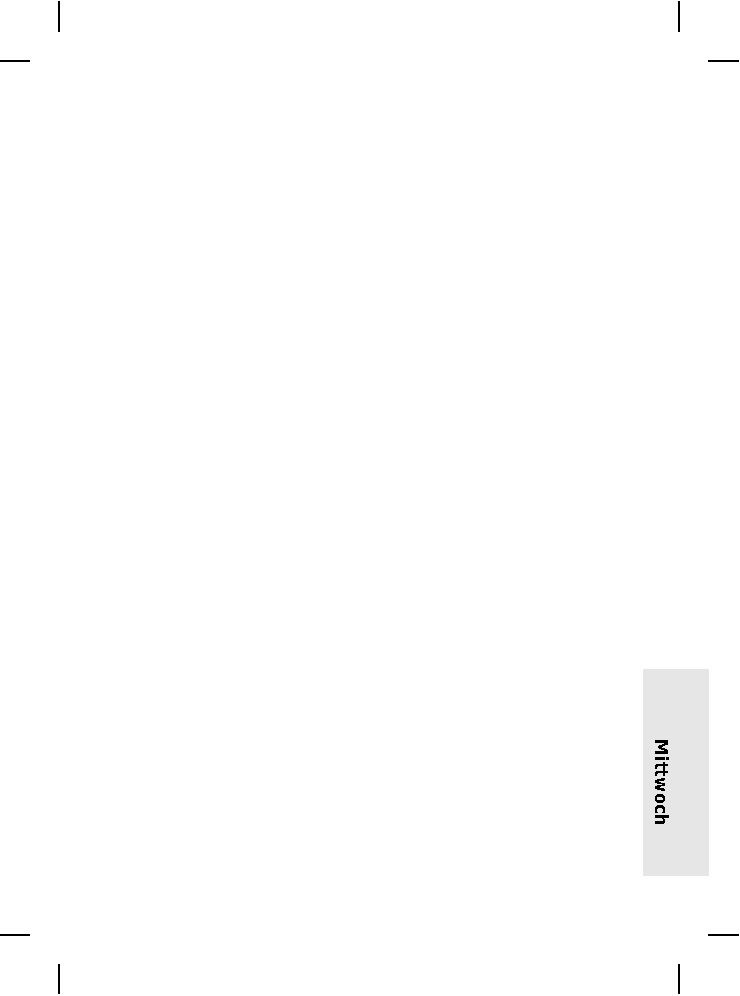
\includegraphics{wallpaper/mittwoch-ungerade.pdf}%
}]{mittwochungerade}
\DeclareNewLayer[background, evenpage,  width=125mm,%
height=169mm, contents={%
  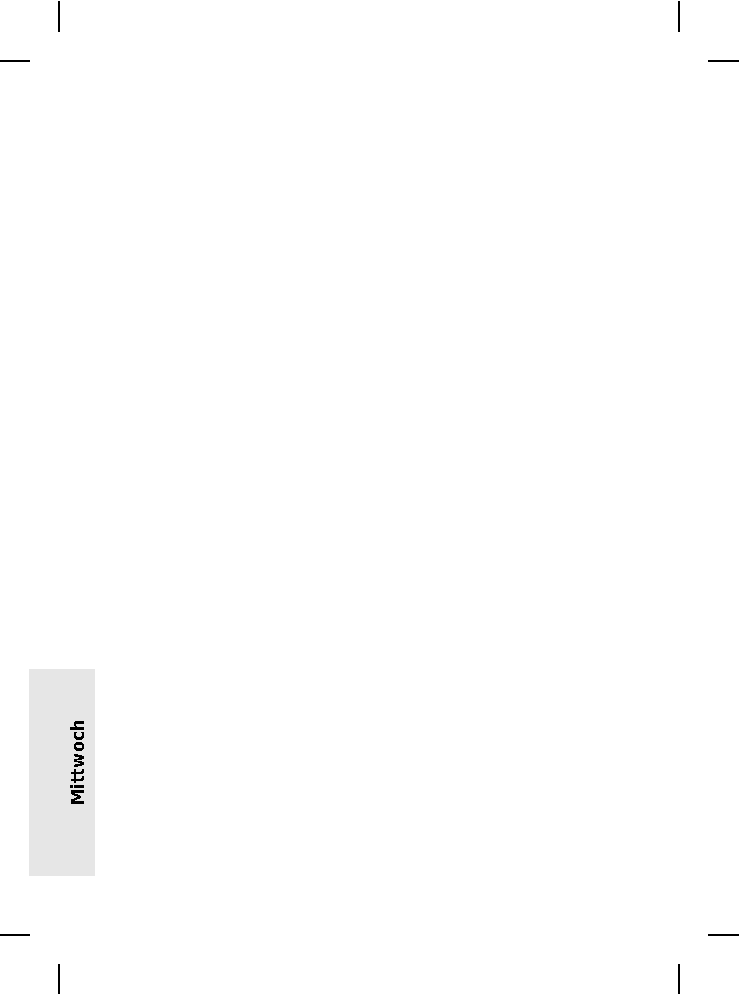
\includegraphics{wallpaper/mittwoch-gerade.pdf}%
}]{mittwochgerade}
\newpairofpagestyles[scrheadings]{mittwoch}{}
\AddLayersAtBeginOfPageStyle{mittwoch}{mittwochgerade}
\AddLayersAtBeginOfPageStyle{mittwoch}{mittwochungerade}
% Donnerstag
\DeclareNewLayer[background, oddpage,  width=125mm,%
height=169mm, contents={%
  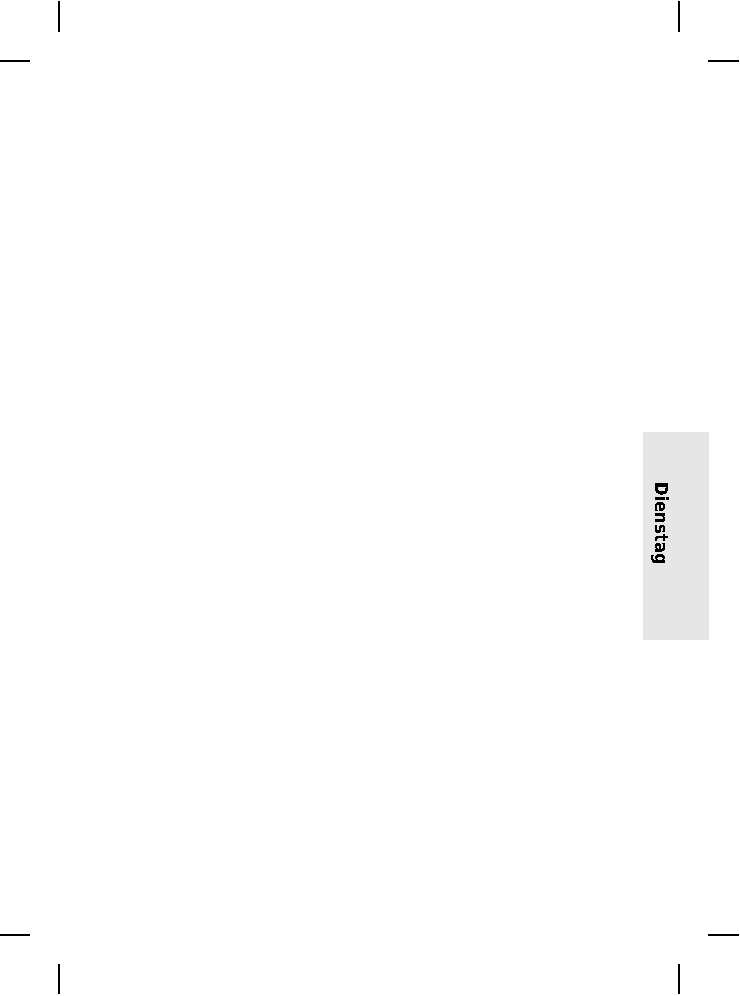
\includegraphics{wallpaper/donnerstag-ungerade.pdf}%
}]{donnerstagungerade}
\DeclareNewLayer[background, evenpage,  width=125mm,%
height=169mm, contents={%
  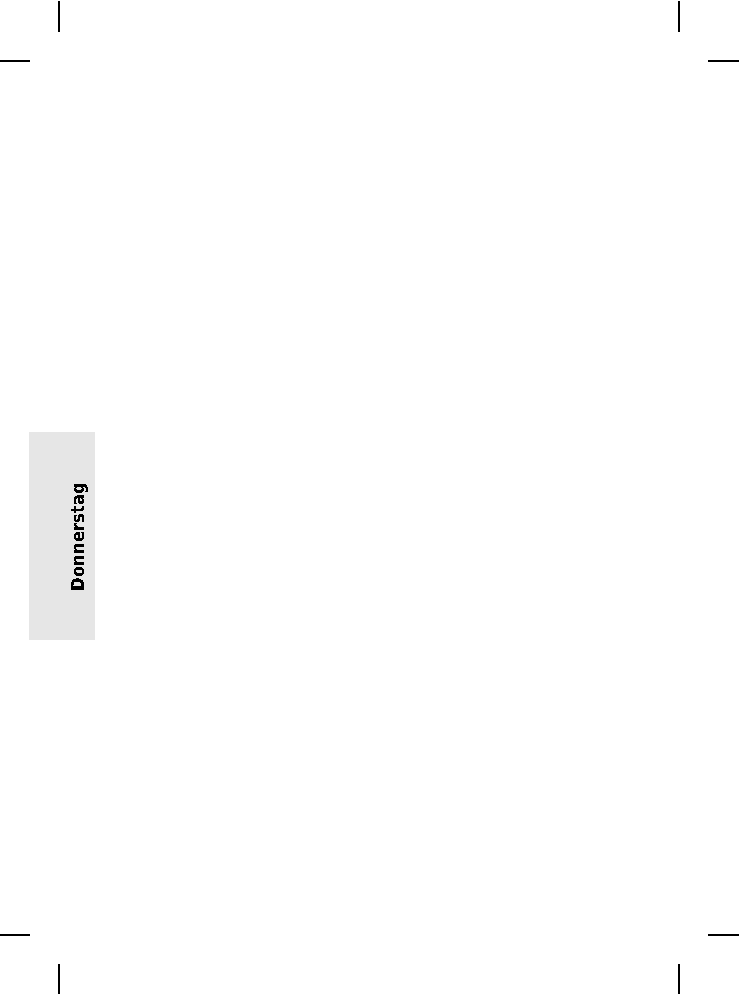
\includegraphics{wallpaper/donnerstag-gerade.pdf}%
}]{donnerstaggerade}
\DeclareNewLayer[background, oddpage,  width=125mm,%
height=169mm, contents={%
  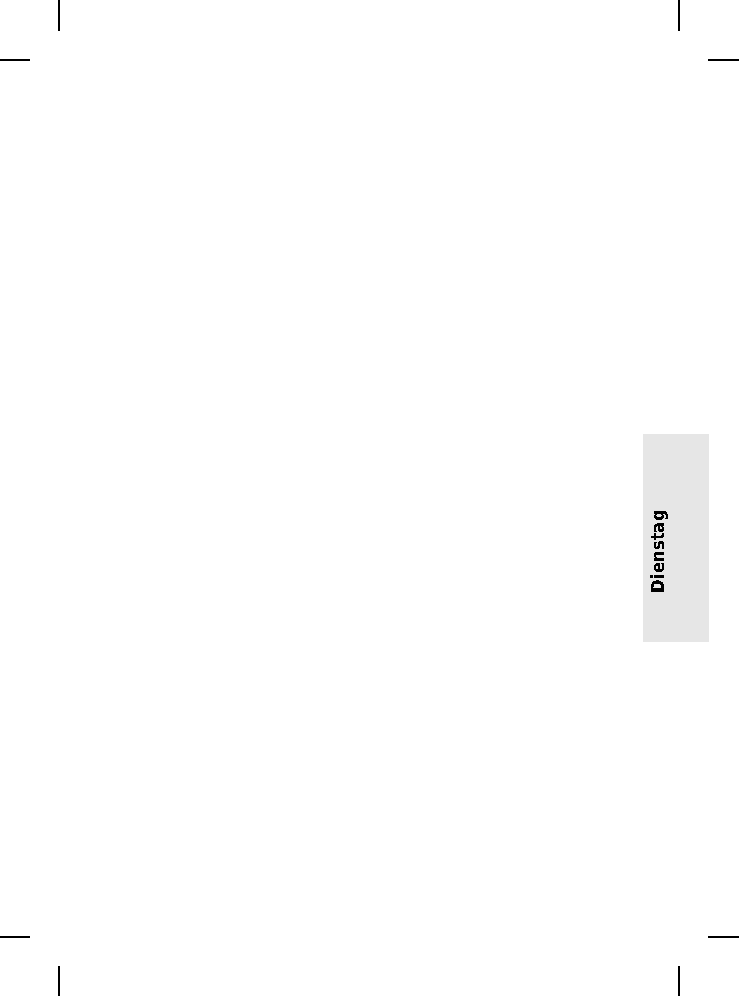
\includegraphics{wallpaper/donnerstag-ungerade-gedreht.pdf}%
}]{donnerstagungeradegedreht}
\newpairofpagestyles[scrheadings]{donnerstag-tabelle}{}
\AddLayersAtBeginOfPageStyle{donnerstag-tabelle}{donnerstaggerade}
\AddLayersAtBeginOfPageStyle{donnerstag-tabelle}{donnerstagungeradegedreht}
\newpairofpagestyles[scrheadings]{donnerstag}{}
\AddLayersAtBeginOfPageStyle{donnerstag}{donnerstaggerade}
\AddLayersAtBeginOfPageStyle{donnerstag}{donnerstagungerade}
% Freitag
\DeclareNewLayer[background, oddpage,  width=125mm,%
height=169mm, contents={%
  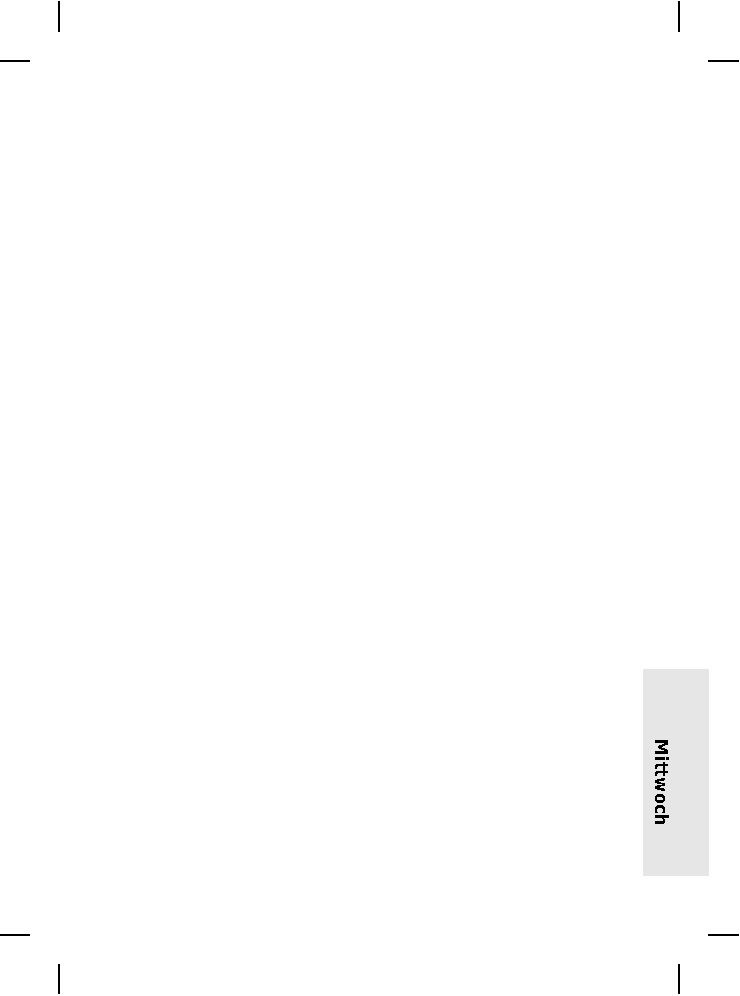
\includegraphics{wallpaper/freitag-ungerade.pdf}%
}]{freitagungerade}
\DeclareNewLayer[background, evenpage,  width=125mm,%
height=169mm, contents={%
  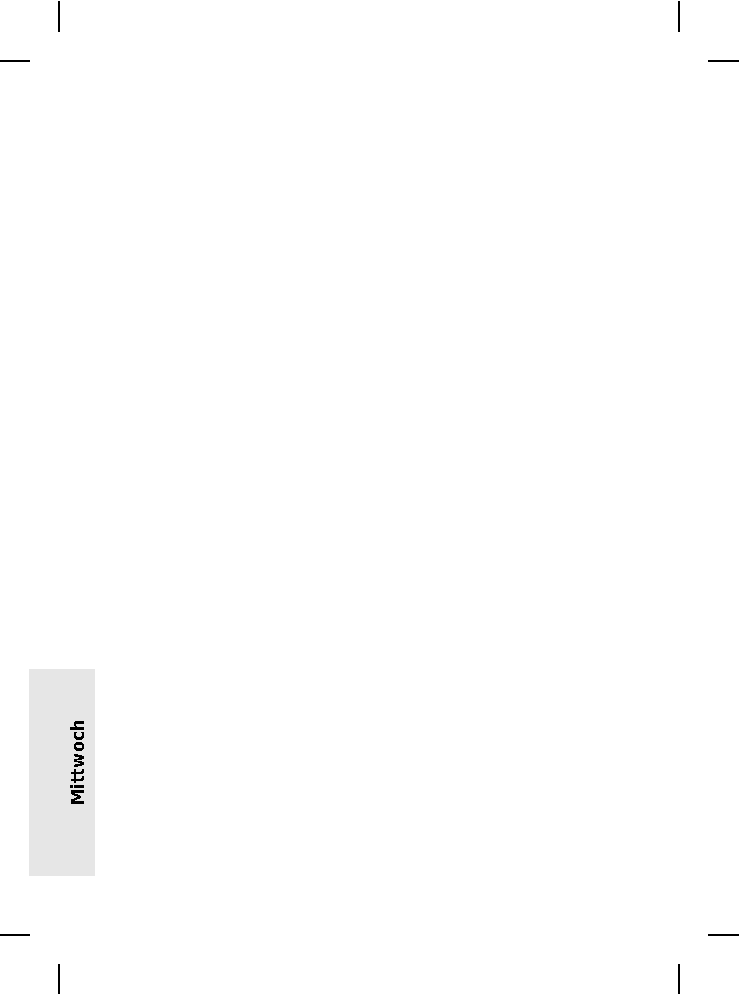
\includegraphics{wallpaper/freitag-gerade.pdf}%
}]{freitaggerade}
\newpairofpagestyles[scrheadings]{freitag}{}
\AddLayersAtBeginOfPageStyle{freitag}{freitaggerade}
\AddLayersAtBeginOfPageStyle{freitag}{freitagungerade}

% \setpagebackground wählt anhand des aktuellen Tages aus, welcher
% Seitenstil verwendet werden soll. Jeder Tag ist ein eigener Seitenstil.
\newcommand{\setpagebackground}{ %
  \ifthenelse{\equal{\konferenztag}{\mittwoch}}{%
    \pagestyle{mittwoch}
  }{}
  \ifthenelse{\equal{\konferenztag}{\donnerstag}}{%
    \pagestyle{donnerstag}
  }{}
  \ifthenelse{\equal{\konferenztag}{\freitag}}{%
    \pagestyle{freitag}
  }{}
}


% zusätzlicher Spaltentyp für die Titeltabelle
\newcolumntype{Y}[1]{>{\RaggedRight\arraybackslash}p{#1}}

%% Längen für Titelboxen
\newlength{\titleboxwidth}
\setlength{\titleboxwidth}{\textwidth}
\advance\titleboxwidth by -6pt

% Befehl zum Setzen von Titelboxen
\newcommand{\setabstract}[6]{
	% 1. Sprecher
	% 2. Titel
	% 3. Untertitel
	% 4. Abstract (Text)
	% 5. Farbe
	% 6. Raum
	%\thispagestyle{scrheadings}
  \setpagebackground
	\setlength\tabcolsep{0pt}
	% \setlength{\fboxsep}{0pt}
	\noindent\fcolorbox{white}{#5}{\parbox{\titleboxwidth}{%
		\noindent\begin{tabu}{X[5L]r}
			\isspeakerempty{#1}{#2}{#6}
			\issubtitleempty{#3}
		\end{tabu}%
	}}
	%
	\isabstractempty{#4}%
	\vspace{0.5em}% Abstand zum nächsten Talk, auch wenn es keinen Abstract gibt
	\setlength\tabcolsep{6pt} % Spaltenpadding wieder auf Default setzen
}

% Setzen des Referenten, falls vorhanden
% Wir gehen davon aus, dass es einen Untertitel nur dann gibt, wenn es auch einen Referenten gibt
\makeatletter
\newcommand{\isspeakerempty}[3]{%
	% Arguments:
	% 1. speaker
	% 2. title
	% 3. room
	\@ifmtarg{#1}{%
			\par\noindent\large \sectfont #2% % Titel
			&
			#3, \talktime
			\tabularnewline
		}
		{
			\emph{#1} % Sprecher
			&
			\talktime
			\tabularnewline
			{\par\noindent\large \sectfont #2}% % Titel
			&
			#3
			\tabularnewline
		}
		
}
\makeatother

% Setzen des Untertitels
% muss ausgelagert und durch \makeatletter umgeben sein
\makeatletter
\newcommand{\issubtitleempty}[1]{%
	\@ifnotmtarg{#1}{\multicolumn{2}{Y{\linewidth}}{\vspace{-0.6em} \noindent\bfseries \normalsize \sectfont #1}\tabularnewline}
}
\makeatother

% Setzen des Abstracts, falls vorhanden
% muss ausgelagert und durch \makeatletter umgeben sein
\makeatletter
\newcommand{\isabstractempty}[1]{%
		\vspace{0.5em}\newline%
		#1 \par% % Abstract
		\vspace{1.5em}% Abstand zum nächsten Talk, auch wenn es einen Abstract gibt
}
\makeatother

% Farben definieren
%\definecolor{eins}{cmyk}{ 0 .18 .06 .10}
\definecolor{eins}{cmyk}{ 0 .13 .04 .08}
\definecolor{zwei}{cmyk}{ .1 0 .17 .05}
\definecolor{hellorange}{cmyk}{ 0 0.13 0.35 0.03}
%\definecolor{aula}{cmyk}{ 0.2 0 0.05 0.13}
\definecolor{aula}{cmyk}{ 0.13 0 0.04 0.11}
\definecolor{geoblau}{cmyk}{ 0.2 .02 0 .01}
\definecolor{dezentrot}{cmyk}{ 0 .17 0.21 .04}
\definecolor{hellgelb}{cmyk}{ 0 .02 0.26 0}
\definecolor{hellgruen}{cmyk}{ 0.05 .0 0.17 0.05}

% Abstract AM HS 9
\newcommand{\abstractNeun}[4]%
{%
	\setabstract{#1}{#2}{#3}{#4}{hellgruen}{AM HS\,9}
}

% Abstract IM HS 13
\newcommand{\abstractDreizehn}[4]%
{%
	\setabstract{#1}{#2}{#3}{#4}{hellgelb}{IM HS\,13}
}

% Abstract IM HS 11
\newcommand{\abstractElf}[4]%
{%
	\setabstract{#1}{#2}{#3}{#4}{geoblau}{IM HS\,11}
}

% Abstract AM HS 10
\newcommand{\abstractZehn}[4]%
{%
	\setabstract{#1}{#2}{#3}{#4}{hellorange}{AM HS\,10}
}

% Workshop STUDLAB
\newcommand{\workshopbox}[3]%
{%
	% 1. Titel
	% 2. Referent
	% 3. HS-Nummer
	\setlength\tabcolsep{0pt}
	\noindent\fcolorbox{white}{dezentrot}{\parbox{\titleboxwidth}{%
			\noindent
			\begin{tabu}{X[5L]r}
				\emph{#2} % Sprecher
				&
				\talktime
				\tabularnewline
				{\noindent\large \bfseries #1}% % Titel
				&
				Workshop #3
				\tabularnewline
			\end{tabu}
		}
	}
	\setlength\tabcolsep{6pt} % Spaltenpadding wieder auf Default setzen
}

% viel zu lang
\newcommand{\zulang}{Dieser Text ist viel zu lang. Dieser Text ist viel zu lang. Dieser Text ist viel zu lang. Dieser Text ist viel zu lang. Dieser Text ist viel zu lang. Dieser Text ist viel zu lang. Dieser Text ist viel zu lang. Dieser Text ist viel zu lang. Dieser Text ist viel zu lang. Dieser Text ist viel zu lang. Dieser Text ist viel zu lang. Dieser Text ist viel zu lang. Dieser Text ist viel zu lang. Dieser Text ist viel zu lang. }

%% Längen für Sponsorenbox
\newlength{\fboxwidth}

\def\workshopsSection{workshopsSection}
\def\abstractsSection{abstractsSection}
\newcommand{\sponsorenbox}[4]{%
  %% Längen für Sponsorenbox
  \setlength{\fboxwidth}{\textwidth}
  \advance\fboxwidth by -7.0pt
  \abstractSponsorenbox{#1}{#2}{#3}{#4}{\workshopsSection}%
}

\newcommand{\sponsorenboxA}[4]{%
  %% Längen für Sponsorenbox
  \setlength{\fboxwidth}{\textwidth}
  \advance\fboxwidth by -10.0pt
  \abstractSponsorenbox{#1}{#2}{#3}{#4}{\abstractsSection}%
}

%% Sponsorenbox
%% 1. Logo
%% 2. Logobreite
%% 3. Anzahl benötigter Zeilen
%% 4. Text
%% 5. Umfeld (\workshopsSection oder \abstractsSection}
\makeatletter
\newcommand{\abstractSponsorenbox}[5]{%
  \setlength{\fboxsep}{4.5pt}%
  \noindent%
  \ifthenelse{\equal{#5}{\workshopsSection}}{%
    \hspace{2.65pt}%
  }{\hspace{-1pt}}%
  \fcolorbox{gray}{white}{\parbox{\fboxwidth}{
    \@ifmtarg{#1}{}{%
      \begin{wrapfigure}[#3]{r}[0pt]{#2}
        \centering\vspace{-1\baselineskip}
        \includegraphics[width=#2]{#1}
      \end{wrapfigure}
    }

    \noindent #4
  }}
  \setlength{\fboxsep}{3pt}
}
\makeatother

% Definitionen für Tagestabellen
\newcolumntype{Z}[1]{>{\RaggedRight\arraybackslash}p{#1}}%
\newcolumntype{C}[1]{>{\Centering\arraybackslash}p{#1}}%
\newcommand{\talk}[2]%
{%
	& \textbf{#1} \newline \emph{#2}
}%
% Titel -- Redner


\newcommand{\workshop}[3]%
{%
	\workshopbox{#1}{#2}{#3}
}%

\newcommand{\otherevent}[1]%
{%
	& \textbf{#1}
}%

\newcommand{\aulaevent}[2]%
{%
	&
	\multicolumn{3}{c}{
		\textbf{#1} (Aula) \par \emph{#2}
	}
}%

\newcommand{\coffeespace}{\vspace{0.4em}}
\newcommand{\workshopspace}{\vspace{0.5em}\\}

% Farben definieren
\definecolor{commongray}{gray}{.9}
%\vspace{-1.2em}
\renewcommand{\arraystretch}{1.4}



\begin{document}
\lsstyle
\usefont{T1}{DejaVuSansCondensed-TLF}{m}{n}
 
% Schneidemarken
% Befehl zum Aufrufen definieren
\newcommand{\cropmarkswallpaper}{%
\CenterWallPaper{1.0}{crop-marks}%
}

\begin{titlepage}
%
\includepdf{deckseite-vektor-mit-schnittmarken}
\end{titlepage}

\cropmarkswallpaper
\selectlanguage{ngerman}
\newpage
% 10:30
\renewcommand{\konferenztag}{\mittwoch}
\newsmalltimeslot{10:30}
\abstractNeun{Dominik Helle}%
{Die Open-Source-Software}%
{Vorstellung ausgewählter Projekte}%
{Vor dem offiziellen Start der Konferenz geben wir einen Einblick in die Welt der Open-Source-Software. Nach einer kleinen Einführung in das Thema stellen sich einige bekannte Open-Source-Projekte gezielt vor.

Die Projekt werden dabei größtenteils von den Entwicklern selbst vorgestellt. Mit dabei sind unter anderem:
OpenLayers, QGIS, MapProxy, Mapbender, GeoServer, GRASS GIS und die PostNAS Suite.}

% 13:00
\newsmalltimeslot{13:00}%
\abstractZehn{Marco Lechner}%
{Eröffnungsveranstaltung der FOSSGIS-Konferenz 2017}%
{}%
{}

\newsmalltimeslot{13:15}%
\abstractZehn{Olaf Knopp}%
{Vortrag des Goldsponsors WhereGroup}%
{}%
{Die WhereGroup freut sich, in diesem Jahr~-- nach 2015 bereits zum zweiten Mal~--
Goldsponsor der FOSSGIS Konferenz zu sein.}

% 13:30
\newsmalltimeslot{13:30}
\abstractZehn{Hans-Jörg Stark}%
{Von proprietärer zu Open-Source-Software}%
{Erfahrungen aus der Verwaltung bei der Migration von proprietärer zu Open-Source-Software im
Web-Mapping-Bereich}%
{Dieser Beitrag stellt den Prozess, die Schwierigkeiten, Chancen und auch die "lessons learnt" vor
beim Wechsel von proprietärer zu Open-Source-Software im Bereich Webmapping/WebGIS.}

\newsmalltimeslot{14:00}%
\abstractZehn{}%
{Lightning Talks Opening}%
{}%
{Geplante Vorträge:\\
OSM Wiki-Tag History -- Alexander Zipf\\
Der FOSSGIS kann auch international -- Till Adams\\
Geopedia -- Michael Schön\\
Freie Software und freie Daten sind heute weitgehend verfügbar -- was fehlt zum Glück? -- Christian
Strobl}

% 15:00
\newtimeslot{15:00}
\abstractNeun{Daniel Koch}%
{GeoServer 2.10/2.11: Status, neue Features und Erweiterungen}%
{}%
{%TODO ergänzen
}

%2017-03-22 15:00:00
\abstractDreizehn{Martin Raifer}%
{OSM-History-Analysen auf Basis von Big-Data-Technologie}%
{}%
{Für tiefgründige OSM-Datenanalysen werden mit unter Full-History-Planet-Dumps benötigt, welche zur
Verarbeitung leider schnell recht unhandlich werden können. Um diese Situation zu verbessern
betreibt die Universität Heidelberg seit Kurzem verteilte Big-Data-Infrastruktur, die den Zugriff
auf die kompletten OSM-History-Daten erleichtert. Damit soll die Forschung an intrinsischen
Datenqualitätsanalysen vorangetrieben, sowie die Entwicklung von neuen Visualisierungen und Tools
ermöglicht werden.}%

\newtimeslot{15:30}
%2017-03-22 15:30:00
\abstractNeun{Dominik Helle}%
{Neues von MapProxy}%
{}%
{Im Vortrag werden neue und unbekannte Funktionen von MapProxy vorgestellt. Hierzu zählen zum
Beispiel die Funktionen zum on-the-Fly transformieren von Karten in Falschfarben und Graustufen,
sowie die Unterstützung des ArcGIS-Cache-Layout.}

\abstractDreizehn{Roland Zink}%
{OSM-basierte Standortmodellierung von Ladesäulen für Elektromobilität am Beispiel des Bayerischen Waldes}%
{}%
{Obwohl die Umstellung des Individualverkehrs von fossilen Treibstoffen auf Elektromobilität große
Vorteile hinsichtlich Klima- und Emissionsschutz bieten würde, stagniert der Absatz von
Elektrofahrzeugen auf niedrigem Niveau. Ein Grund hierfür ist die mangelnde Ladeinfrastruktur
insbesondere in ländlichen Räumen. Der Vortrag präsentiert einen GIS-basierten Ansatz, wie sich mit
frei verfügbaren Geo- und Nutzungsdaten Standorte mit hohem Ladebedarf ermitteln lassen.}

\newtimeslot{16:00}
\abstractNeun{Marc Jansen}%
{OpenLayers}%
{Stand, Neues und Zukünftiges}%
{}

\abstractDreizehn{Michael Reichert}%
{Qualitätssicherung mit Vektortiles}%
{}%
{Bisher existente Qualitätssicherungswerkzeuge, die nicht auf ein spezielles Thema fokussiert sind,
  können ihre Daten meist nur täglich aktualisieren, denn sie prozessieren jedes Mal den gesamten
  Planet. In einer Zeit, in der öffentliche Tileserver minütliche Diffs beziehen, sind tägliche
  Updates eigentlich zu langsam.

Mit einer Vektortile-basierten Architektur sind häufigere Updates möglich, denn es werden – wie bei
einem Tileserver – nur die Tiles neu prozessiert, die sich geändert haben. Die Schwierigkeit liegt
darin, den inhaltlichen und räumlichen Umfang der Vektortiles festzulegen.}

\newtimeslot{17:00}
\abstractNeun{Horst Reinecke}%
{Lassen wir einmal eine Statistik drüber laufen ...}%
{%Interaktive Visualisierung und Analyse geostatistischer Telemetriedaten am Beispiel freilebender Rothirsche
}%
{Am Beispiel freilebender telemetrierter Rothirsche wird die interaktive Darstellung und Auswertung
  tagesaktueller Daten demonstriert. Browserbasiert erfolgt sowohl eine kartenmäßige Darstellung,
  als auch eine deskriptive statistische Auswertung der Daten.
%  Vom Anwender werden dabei weder
%  Web-GIS- noch statistische Funktionalitäten verlangt.
  Die Anwendung läuft plattformunabhängig auf
  PCs und auf Android-Tablets.

Realisiert wird die Anwendung mit der Statstiksprache R, dem Package Shiny und einiger weiterer
Packages. Der Vortrag zeigt sowohl Funktionalitäten als auch einige technische Voraussetzungen.}

\abstractDreizehn{Falk Zscheile}%
{Lizenzinkompatibilitäten bei Open Data Lizenzen}%
{}%
{Im Bereich Open Data existiert für den Lizenzgeber ein breiter Gestaltungsspielraum. Die Kehrseite
  dieser Handlungsfreiheiten bei der Lizenz sind Lizenzinkompatibilitäten. Nicht alles was Open Data
  ist, darf auch miteinander kombiniert werden.

Der Vortrag erklärt die Hintergründe von Lizenzinkompatibilitäten, gibt Hinweise, wie man diese
erkennen kann und welche Handlungsoptionen es gibt.}

\newtimeslot{17:30}
\abstractNeun{Stefan Kuethe}%
{Shine on R}%
{Geospatial data processing the /Ahh/R way}%
{Dieser Vortrag gibt einen Überblick über die Möglichkeiten der Vearbeitung räumlicher Daten mit der
  Open-Source-Programmiersprache R. Dabei wird zuerst eine kurze Einführung in R (vor allem die Art
  und Weise, wie R mit Daten umgeht) gegeben. Danach werden die gängigsten R-Pakete zum Umgang mit
  räumlichen Daten anhand von Beispielen vorgestellt. Abschließend wird die Verwendung von
  Javascript-Bibliotheken wie Leaflet in R zur Implementierung interaktiver (Geo)-Webapplikationen
  in wenigen Zeilen Code und die Möglichkeiten der Einbindung des R-Ökosystems in QGIS und
  Docker-Umgebungen gezeigt.}

\abstractDreizehn{Hartmut Holzgraefe}%
{Druckbare Karten im Web erzeugen}%
{MapOSMatic und MyOSMatic}%
{% Platz für 320 Zeichen
  MapOSMatic ist ein webbasierter Druckdienst mit dem großflächige oder mehrseitige OSM-Karten im
  PDF-, SVG- und PNG-Format erzeugt werden können. Neben verschiedenen Kartenstilen und Overlays
  bietet MapOSMatic auch die Möglichkeit mehrseitige Atlanten zu erzeugen und Karten mit einem
  Straßenindex zu versehen.
}

\newtimeslot{18:00}
\abstractNeun{}%
{Lightning Talks I}%
{}%
{Routenplanung durch Flächen -- Jakob Miksch\\
Interaktive Visualisierung von Geodaten in Jupyter Notebooks -- Johannes Kröger\\
Summer of Code -- Tobias Knerr\\
osm\_address\_db -- Stand der Dinge -- Christopher Lorenz}

%2017-03-22 19:00:00
\abstractDreizehn{Axel Heinemann}%
{Erstellung von Karten mit OSM-Daten}%
{}%
{Sollen Informationen in einer Karte visualisiert werden, wird meistens eine
Hintergrundkarte als Basisinformation zur besseren Orientierung benötigt. In
einem QGIS-Projekt wurden verschiedene Möglichkeiten eine Hintergrundkarte zu
erstellen und zu editieren, getestet und auf Eignung geprüft. Beleuchtet werden
die amtliche digitale TK, Web Anwendungen sowie QGIS-Plugins. Ein geeigneter
Weg OSM-Daten in QGIS zu nutzen wird am Beispiel-Projekt gezeigt.}

\newsmalltimeslot{18:30}
\abstractDreizehn{Astrid Emde}{\label{bof-mittwoch}%
Mapbender3-Anwendertreffen}{}{}

\newpage



\end{document}
